\documentclass[11pt]{article}\usepackage[]{graphicx}\usepackage[]{color}
% maxwidth is the original width if it is less than linewidth
% otherwise use linewidth (to make sure the graphics do not exceed the margin)
\makeatletter
\def\maxwidth{ %
  \ifdim\Gin@nat@width>\linewidth
    \linewidth
  \else
    \Gin@nat@width
  \fi
}
\makeatother

\definecolor{fgcolor}{rgb}{0.345, 0.345, 0.345}
\newcommand{\hlnum}[1]{\textcolor[rgb]{0.686,0.059,0.569}{#1}}%
\newcommand{\hlstr}[1]{\textcolor[rgb]{0.192,0.494,0.8}{#1}}%
\newcommand{\hlcom}[1]{\textcolor[rgb]{0.678,0.584,0.686}{\textit{#1}}}%
\newcommand{\hlopt}[1]{\textcolor[rgb]{0,0,0}{#1}}%
\newcommand{\hlstd}[1]{\textcolor[rgb]{0.345,0.345,0.345}{#1}}%
\newcommand{\hlkwa}[1]{\textcolor[rgb]{0.161,0.373,0.58}{\textbf{#1}}}%
\newcommand{\hlkwb}[1]{\textcolor[rgb]{0.69,0.353,0.396}{#1}}%
\newcommand{\hlkwc}[1]{\textcolor[rgb]{0.333,0.667,0.333}{#1}}%
\newcommand{\hlkwd}[1]{\textcolor[rgb]{0.737,0.353,0.396}{\textbf{#1}}}%
\let\hlipl\hlkwb

\usepackage{framed}
\makeatletter
\newenvironment{kframe}{%
 \def\at@end@of@kframe{}%
 \ifinner\ifhmode%
  \def\at@end@of@kframe{\end{minipage}}%
  \begin{minipage}{\columnwidth}%
 \fi\fi%
 \def\FrameCommand##1{\hskip\@totalleftmargin \hskip-\fboxsep
 \colorbox{shadecolor}{##1}\hskip-\fboxsep
     % There is no \\@totalrightmargin, so:
     \hskip-\linewidth \hskip-\@totalleftmargin \hskip\columnwidth}%
 \MakeFramed {\advance\hsize-\width
   \@totalleftmargin\z@ \linewidth\hsize
   \@setminipage}}%
 {\par\unskip\endMakeFramed%
 \at@end@of@kframe}
\makeatother

\definecolor{shadecolor}{rgb}{.97, .97, .97}
\definecolor{messagecolor}{rgb}{0, 0, 0}
\definecolor{warningcolor}{rgb}{1, 0, 1}
\definecolor{errorcolor}{rgb}{1, 0, 0}
\newenvironment{knitrout}{}{} % an empty environment to be redefined in TeX

\usepackage{alltt}
\usepackage[top=1.00in, bottom=1.0in, left=1.1in, right=1.1in]{geometry}
\renewcommand{\baselinestretch}{1.1}
\usepackage{graphicx}
\usepackage{natbib}
\usepackage{gensymb}
\usepackage{amsmath}
\usepackage{lineno}


\def\labelitemi{--}
\parindent=0pt
\IfFileExists{upquote.sty}{\usepackage{upquote}}{}
\begin{document}
\bibliographystyle{/Users/Lizzie/Documents/EndnoteRelated/Bibtex/styles/besjournals}
\renewcommand{\refname}{\CHead{}}
\begin{flushright}
Version dated: \today
\end{flushright}
\bigskip
\medskip
\begin{center}

\noindent{\Large {\bf Limiting cues: How spring warming, winter chilling and daylength will shape climate change responses}}\\ 
\bigskip

\noindent {\normalsize \sc
The lab as it was in 2017$^{1,2}$}\\ % Ailene, Cat, Dan, Lizzie, Nacho
\noindent {\small \it
$^1$ Arnold Arboretum of Harvard University, 1300 Centre Street, Boston, Massachusetts, 02131, USA\\
$^2$ Organismic \& Evolutionary Biology, Harvard University, 26 Oxford Street, Cambridge, Massachusetts, 02138, USA\\
$^3$ Forest \& Conservation Sciences, Faculty of Forestry, University of British Columbia, 2424 Main Mall, Vancouver, BC V6T 1Z4}\\
\end{center}

\section{Overview of OSPREE}
Studies versus papers ... how many crops versus wild species ....

\section{Trends in experimental treatments over space}



The actual cues studied varied across latitude with a general trend toward examining more extreme values at higher latitudes. Thus, forcing and chilling treatments decline 0.1$\degree$C per 1 $\degree$ latitude (for forcing, min is -0.1, for max it's -0.06, see Fig \ref{fig:lat}; for chilling it's -0.06 for min and -0.09 for max); and the maximum studied photoperiod increases with latitude (0.09 hr per degree $\degree$ latitude). 

\begin{figure}[t!]
\centering
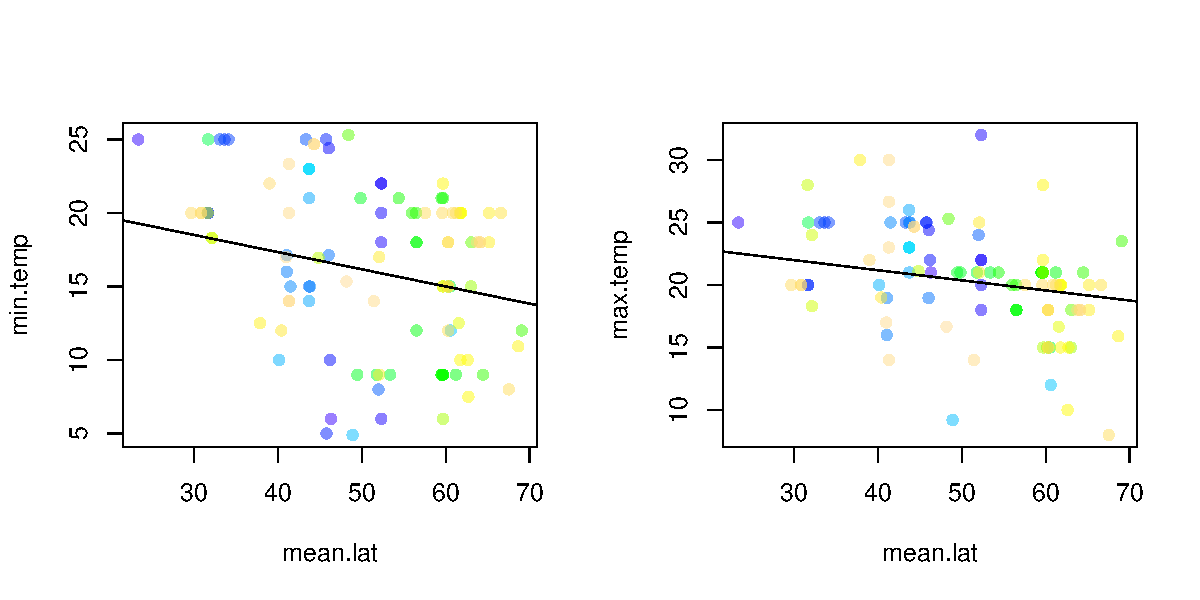
\includegraphics[width=1\textwidth]{..//..//analyses/limitingcues/figures/tempxlatminmaxcorr.pdf}
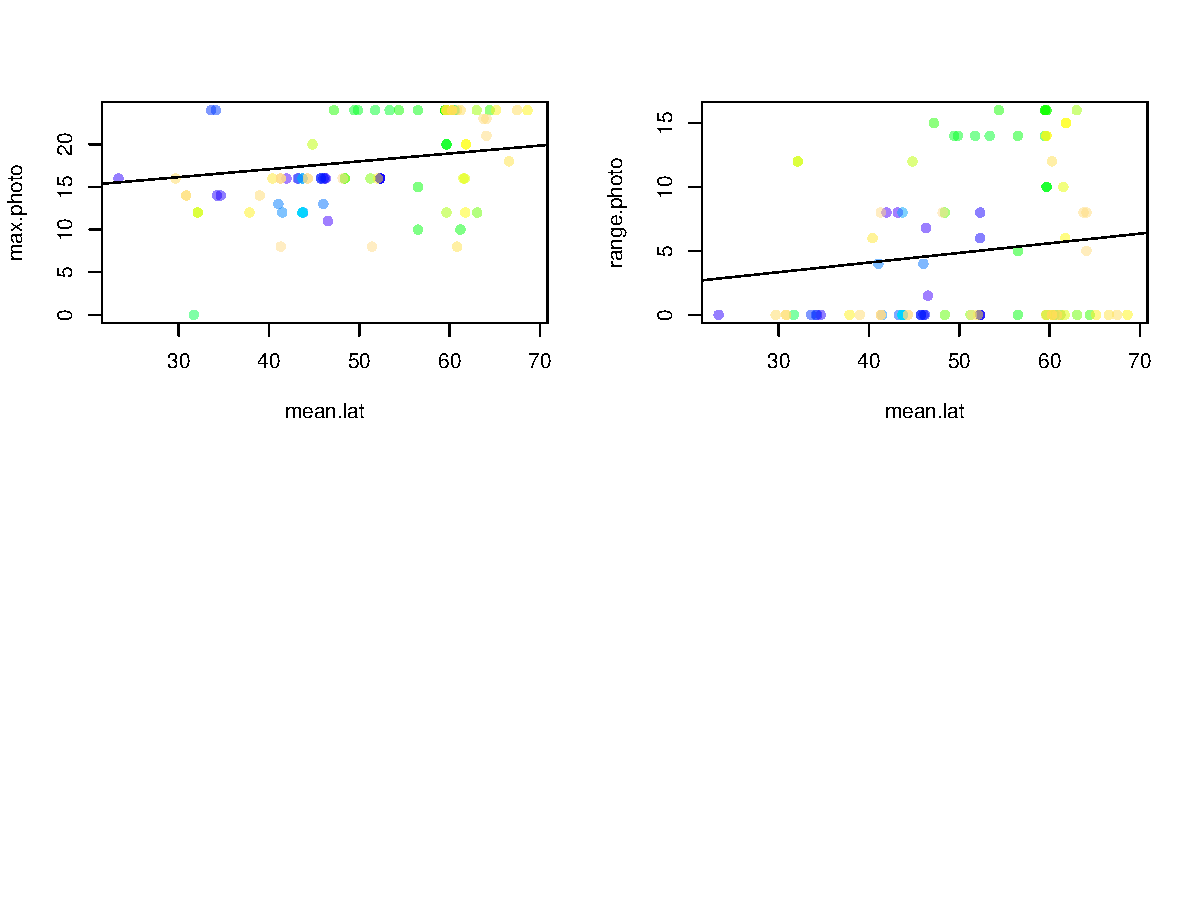
\includegraphics[width=1\textwidth]{..//..//analyses/limitingcues/figures/photoxlatcorr2plots.pdf}
\caption{Some correlations with latitude plots.}
  \label{fig:lat}
\end{figure}

\end{document}

\clearpage

